\documentclass{article}
\usepackage{graphicx}

\begin{document}

\title{COS 314 Assignment 1}
\author{Thato Kalagobe}
\date{\today}
\maketitle

\section{Iterated Local Search (ILS)}
Iterated Local Search (ILS) is a heuristic that solves the Traveling Salesman Problem (TSP) for a set of campuses in this scenario.
\begin{itemize}
    \item \textbf{Initial Solution Generation}: The initial solution is generated by creating a random route between the campuses.
    \item \textbf{Hill Climbing}: This is the local search method used. It iteratively swaps two campuses in the route and accepts the new route if it improves the total distance.
    \item \textbf{Variable Neighbourhood Search (VNS)}: This method shakes the current solution by swapping two campuses and then applies hill climbing to the new solution.
    \item \textbf{Perturbation}: This method is used to escape local optima. It randomly swaps two campuses in the best solution found so far.
    \item \textbf{Run Method}: The VNS and perturbation methods are applied in a loop for a specified number of iterations (1000 in this case).
\end{itemize}

\section{Simulated Annealing (SA)}
Simulated Annealing (SA) is a method that also solves the TSP for a set of campuses in this scenario.
\begin{itemize}
    \item \textbf{Initial Temperature (T0)}: The initial temperature is set to 10000.
    \item \textbf{Cooling Rate}: The cooling rate, which determines how fast the temperature decreases, is set to 0.003.
    \item \textbf{Acceptance Probability Function}: This function determines whether a new solution (neighbour) should be accepted based on the current solution, the neighbour’s cost, and the current temperature.
    \item \textbf{Run Method}: The algorithm repeatedly generates new neighbours and updates the current solution and best solution found so far based on the acceptance probability. The temperature is decreased in each iteration until it reaches 1.
\end{itemize}
Both programs use a cost matrix to represent the distances between the campuses and calculate the total distance of a route. They include methods to get the best route and its total distance. The run times of the programs are calculated and printed out at the end. The best routes are printed out as a sequence of campus names. The programs are designed to always start and end at the “Hatfield” campus.

\section{Table of Results}
\begin{table}[h]
\centering
\begin{tabular}{|l|p{5cm}|p{5cm}|}
\hline
\textbf{Problem Set} & \textbf{ILS} & \textbf{SA} \\ \hline
Best Solution (route) & Hatfield $\rightarrow$ Prinsof $\rightarrow$ Mamelodi $\rightarrow$ Groenkloof $\rightarrow$ Hillcrest $\rightarrow$ Hatfield & Hatfield $\rightarrow$ Hillcrest $\rightarrow$ Groenkloof $\rightarrow$ Prinsof $\rightarrow$ Mamelodi $\rightarrow$ Hatfield \\ \hline
Objective Function Val & 81 & 81 \\ \hline
Runtime & 62.203791 ms & 67.602333 ms \\ \hline
Av Obj Func. & 81 & 81 \\ \hline
\end{tabular}
\caption{Table of results}
\end{table}

\section{Graphical Plot Representation}
The graphical plot representation is presented on page 3.

\begin{figure}
    \centering
    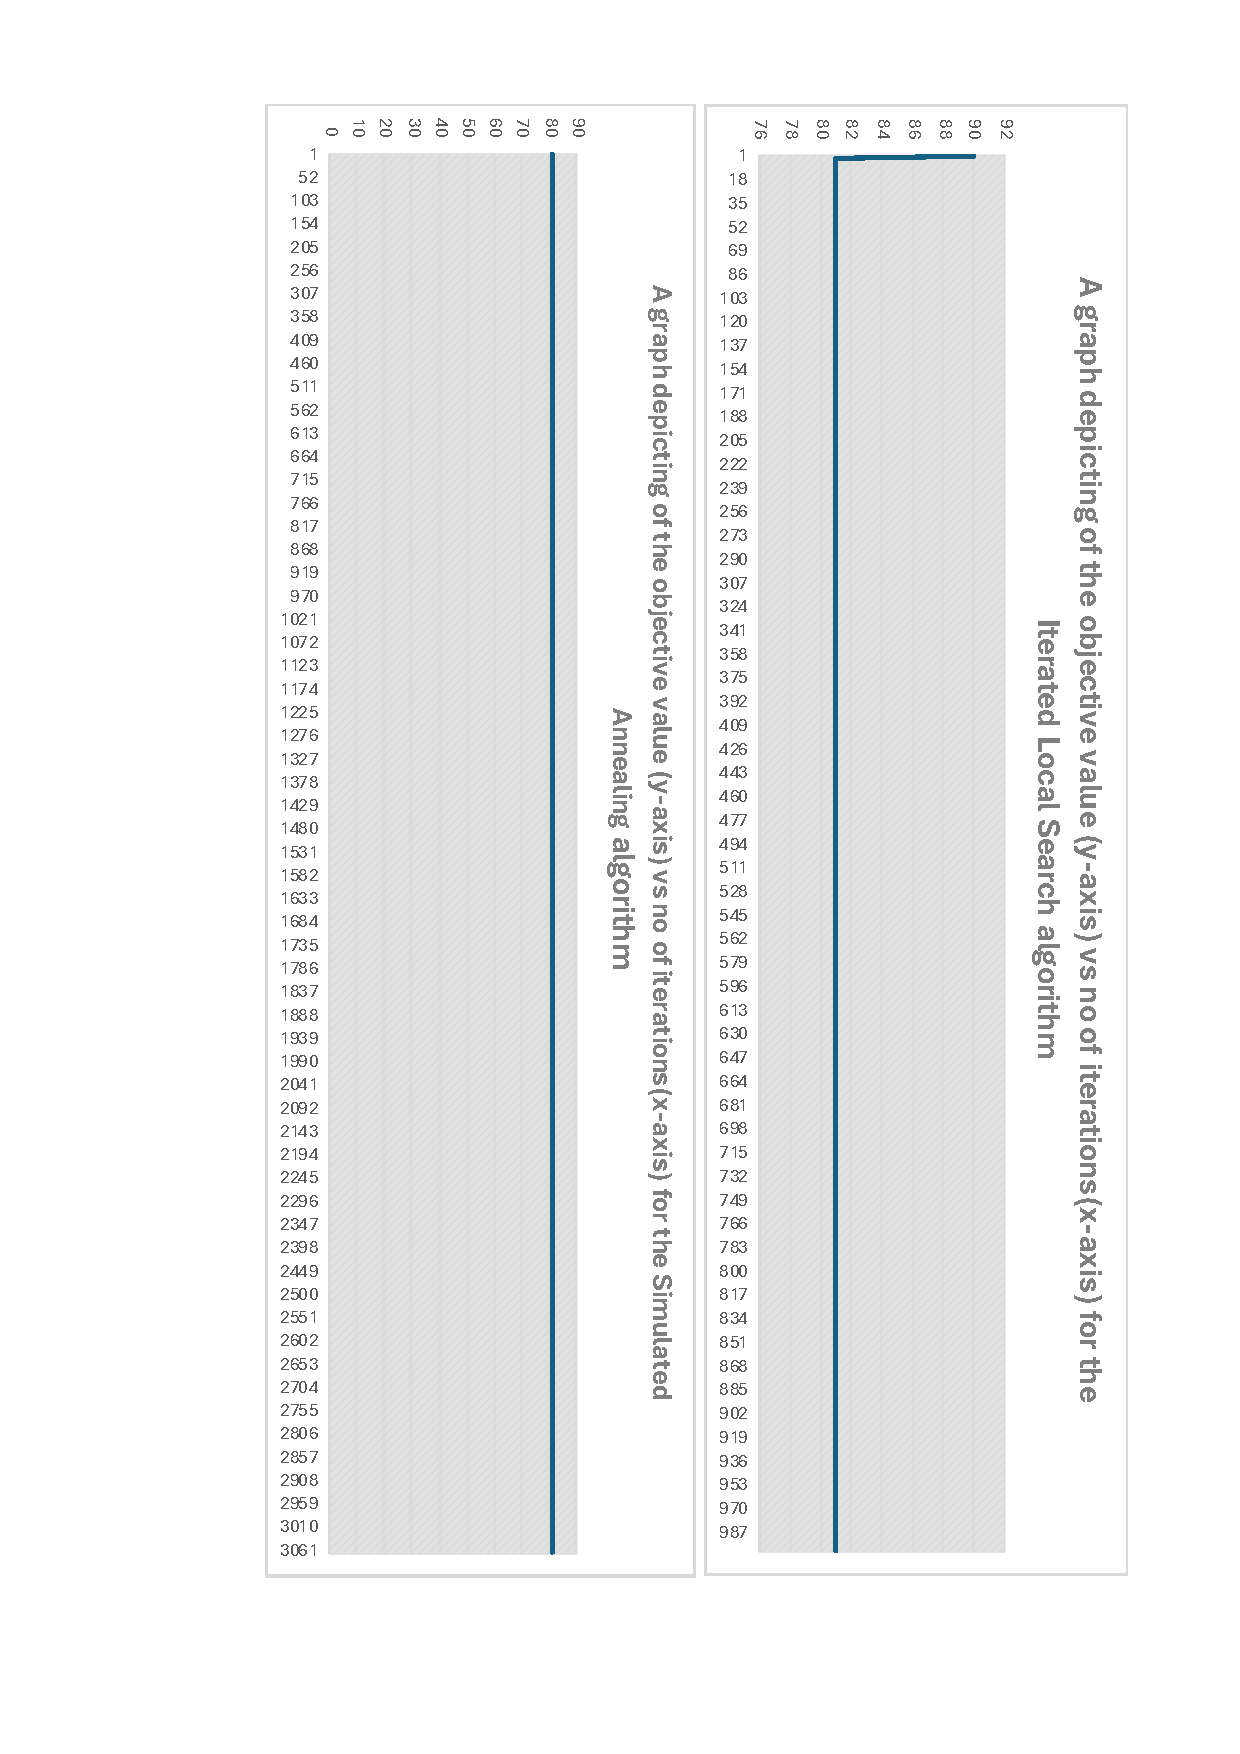
\includegraphics[width=1\textwidth]{graphical_plot_diagram.pdf}
    \caption{Two line graphs representing the objective value vs number of iterations for the Iterated Local Search and Simulated Annealing respectively}
    \label{fig:excel_graph}
\end{figure}

\section{Discussion and Conclusion}
Both Iterated Local Search (ILS) and Simulated Annealing (SA) have found solutions with the same objective function value of 81. This indicates that both algorithms are capable of finding equally good solutions for this problem instance. ILS has a slightly faster runtime (62.203791 ms) compared to SA (67.602333 ms). This suggests that ILS may be more time efficient. The routes derived from ILS and SA are different but lead to the same objective function value. This shows that there can be multiple good solutions to the problem and both algorithms are capable of exploring different parts of the solution space. In conclusion, both ILS and SA have performed well on the problem. While ILS was slightly faster, both algorithms found solutions of equal quality.

\end{document}
